\documentclass[a4paper,12pt]{article}
\usepackage[english]{babel}
\usepackage[T1]{fontenc}
\usepackage[dvips]{graphicx}
\usepackage{times}
\usepackage{epsfig}
\usepackage{color}
\usepackage[urlcolor=blue, colorlinks=true, bookmarks=true, bookmarksnumbered=true]{hyperref}

\usepackage{fancyhdr} 
\pagestyle{fancy} 

\rfoot{SALOMON}


%ustawienie wielkosci akapitu
%\setlength{\parindent}{0mm}
%%odst�p mi�dzy akapitami
%\setlength{\parskip}{2mm}

%ustawienia rozmiaru tekstu
    \textwidth 16cm
    \textheight 24cm 
    \topmargin -15mm
    \evensidemargin-3mm
    \oddsidemargin -3mm
    


\title{Introduction to Salomon}

\author{Nikodem Jura \emph{(nico@icslab.agh.edu.pl)}
        \\
        Krzysztof Rajda \emph{(krzycho@student.uci.agh.edu.pl)}
        }                     

\begin{document}

\maketitle
%wylaczenie numerowania na I stronie
\thispagestyle{empty}

\begin{center}
\href{http://salomon.iisg.agh.edu.pl}{http://salomon.iisg.agh.edu.pl}
\end{center}

\pagebreak
\section{Intro}

Salomon is a system for extracting knowledge out of data using \emph{Knowledge Mining} methodology.

\subsection{Goal}

The goal of this project is to create a friendly environment for creating, controlling and effective performing of tasks and storing collected knowledge.

\subsection{Assumptions}

Basic design objectives:
\begin{itemize}
	\item \textbf{all functionality in plug-ins.}
	
	The core of the system should be as light as possible. Its goal is to create an environment for realizing the functionality provided with the plug-ins.
	
	\item \textbf{open architecture.}
	
	Inserting a middle tier between database and plug-ins. Its goal is to hide the details of how the data is organized. Architecture openness gives the possibility to extend this tier.
	
	\item \textbf{platform independence.}
	
	System should be platform independent and easily portable. Thus each part of the system can be run on different operating systems.
	\item \textbf{possibility of using the results of some task by consequent tasks.}
	\item \textbf{ easy adaptation of the functionality contained in \emph{Vinlen}.}
	
	Project has been originally designed to be a platform for running the logics implemented in \emph{Vinlen} program,
	created under supervision of Prof. Ryszard Michalski
	
\end{itemize}

\begin{figure}[ht]
	\centering
		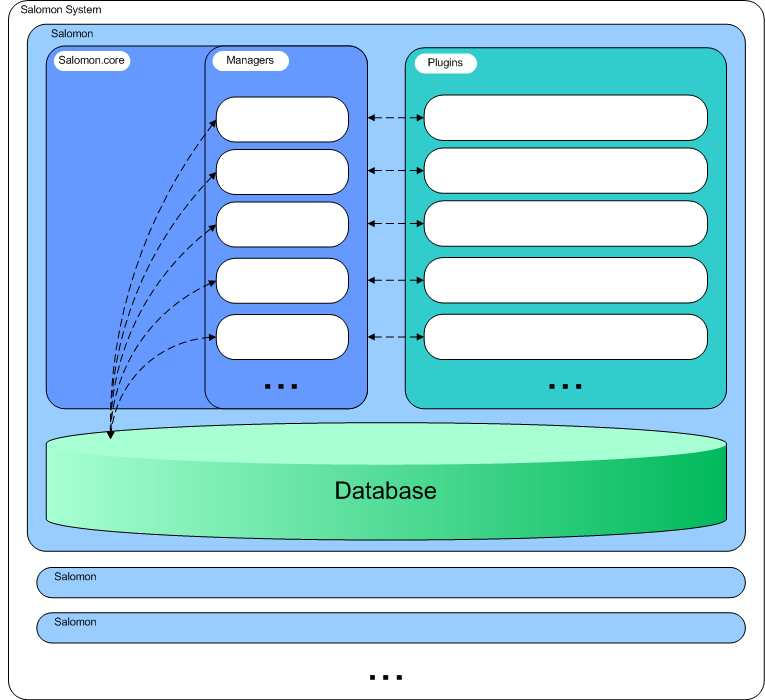
\includegraphics[width=0.70\textwidth]{../documentation/img/uml/arch.jpg}
	\caption{System architecture}
\end{figure}

\newpage
\section{Knowledge processing}

\subsection{Graph}

Discovering knowledge is an iterative, divided into stages, process. Stages can form cycles. 
During each stage the knowledge is processed. Knowledge discovering process can be directed according to the user's preferences. Each stage forms a closed whole. Some stages are separate, so they can be performed concurrently. Salomon's architecture enables support for distributed (and this implies concurrent) processing of those stages and synchronizing their results.

The representation of the stage in Salomon is a \emph{task}. Each task may have a few predecessors and consequents. Simply speaking, tasks can be organized in a form of a graph.

The task is defined as a triple:
\begin{itemize}
	\item algorithm (provided in a form of a plug-in)
	\item data which controls the algorithm
	\item entry data, out of which the algorithm extracts the knowledge
\end{itemize}

\begin{figure}[ht]
	\centering
		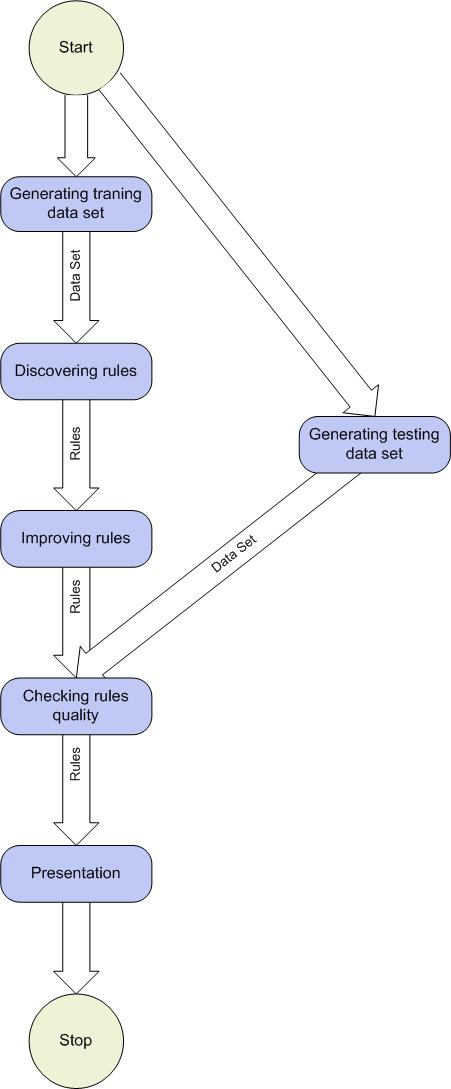
\includegraphics[height=0.4\textheight]{../documentation/img/concept/WorkflowGraph.jpg}
	\caption{General workflow}
	\label{fig:WorkflowGraph}
\end{figure}

\subsection{Task}

The task does not have to be limited to the data, provided by the previous task. Each task has access to the whole currently gathered knowledge and to all data. 

In the output or input of each task there can be data (in case of algorithms, which filters and organize data), knowledge or both of these at the same time.
\begin{itemize}
	\item data \begin{math}\Rightarrow \end{math} data - this case occurs most often when we want to create training or test sets
	\item data \begin{math}\Rightarrow \end{math} knowledge - typical example of knowledge mining: we are given with data, and return knowledge
	\item data + knowledge \begin{math}\Rightarrow \end{math} data - this case occurs when we want to use collected knowledge on the given data
	\item knowledge \begin{math}\Rightarrow \end{math} knowledge
\end{itemize}

\subsection{Differences to Vinlen}

Salomon is meant to eliminate the limits of original \emph{Vinlen} by introducing:
\begin{itemize}
	\item queuing of tasks
	\item distribution
	\item concurrency
	\item extendability (plug-ins mechanism)
	\item portability (Java\texttrademark, Firebird)
\end{itemize}

\section{Acknowledgments}

	Inspiration for creating project ,,Salomon,, was the presentation shown by Prof. Ryszard Michalski, which concerned the system \emph{Vinlen}. 

\end{document}
